\subsection{O Papel da Saliência Temática na Influência do Lobby}

A Hipótese 3 postula que, em temas de maior saliência, o lobby exercido por organizações não empresariais (como as \acrshort{ong}s) tem uma maior probabilidade de influenciar a atividade legislativa dos \acrshort{mpe}s em comparação com o lobby de organizações empresariais. A lógica subjacente é que, quando um tema está sob intenso escrutínio público, os parlamentares se tornam mais sensíveis a argumentos que ressoam com a opinião pública e a interesses difusos, frequentemente representados por \acrshort{ong}s.

Para testar esta hipótese, mantivemos a estrutura do modelo \acrshort{ppml} com efeitos fixos, garantindo a consistência com as análises anteriores. A principal diferença metodológica foi a introdução de uma variável para capturar a saliência de um tema e a sua interação com os diferentes tipos de lobistas.

A saliência foi operacionalizada como uma proxy baseada na intensidade da atividade de lobby, uma abordagem que encontra respaldo na literatura \cite{baumgartner2010agendas}. Especificamente, criamos uma variável (salience\_std) que mede o volume total de reuniões de lobby dentro de cada domínio temático para cada período mensal, padronizada para ter média zero e desvio padrão um. Um valor mais alto nesta variável indica que um tema atraiu mais atenção de todos os grupos de interesse, sendo, portanto, considerado mais saliente.

O modelo econométrico foi então especificado para incluir termos de interação entre cada categoria de lobista (Empresa, \acrshort{ong}, Outros) e a variável de saliência, apresentado na Equação \ref{eq:modelo_h3}. Esta especificação permite-nos estimar como o efeito marginal de uma reunião de cada tipo de ator varia em função do nível de saliência do tema. Os resultados da regressão estão sumarizados na Tabela \ref{tab:h3_interaction} e visualizados no gráfico de efeitos marginais na Figura \ref{fig:h3_marginal_effects}.

\begin{table}
\centering
\begin{talltblr}[         %% tabularray outer open
entry=none,label=none,
note{}={+ p \num{< 0.1}, * p \num{< 0.05}, ** p \num{< 0.01}, *** p \num{< 0.001}},
]                     %% tabularray outer close
{                     %% tabularray inner open
colspec={Q[]Q[]},
column{2}={}{halign=c,},
column{1}={}{halign=l,},
hline{10}={1-2}{solid, black, 0.05em},
}                     %% tabularray inner close
\toprule
& PPML com Interação (H3) \\ \midrule %% TinyTableHeader
Empresa (base) & \num{0.035}*** \\
& (\num{0.006}) \\
ONG (base) & \num{0.090}*** \\
& (\num{0.006}) \\
Outros (base) & \num{0.032}** \\
& (\num{0.010}) \\
Empresa x Saliência & \num{-0.022}*** \\
& (\num{0.005}) \\
Num.Obs. & \num{600237} \\
R2 & \num{0.253} \\
RMSE & \num{0.56} \\
Std.Errors & by: cl\_dt \\
FE: fe\_ct & X \\
FE: fe\_pt & X \\
FE: fe\_dt & X \\
\bottomrule
\end{talltblr}
\end{table}



\begin{figure}[htbp]
    \centering
    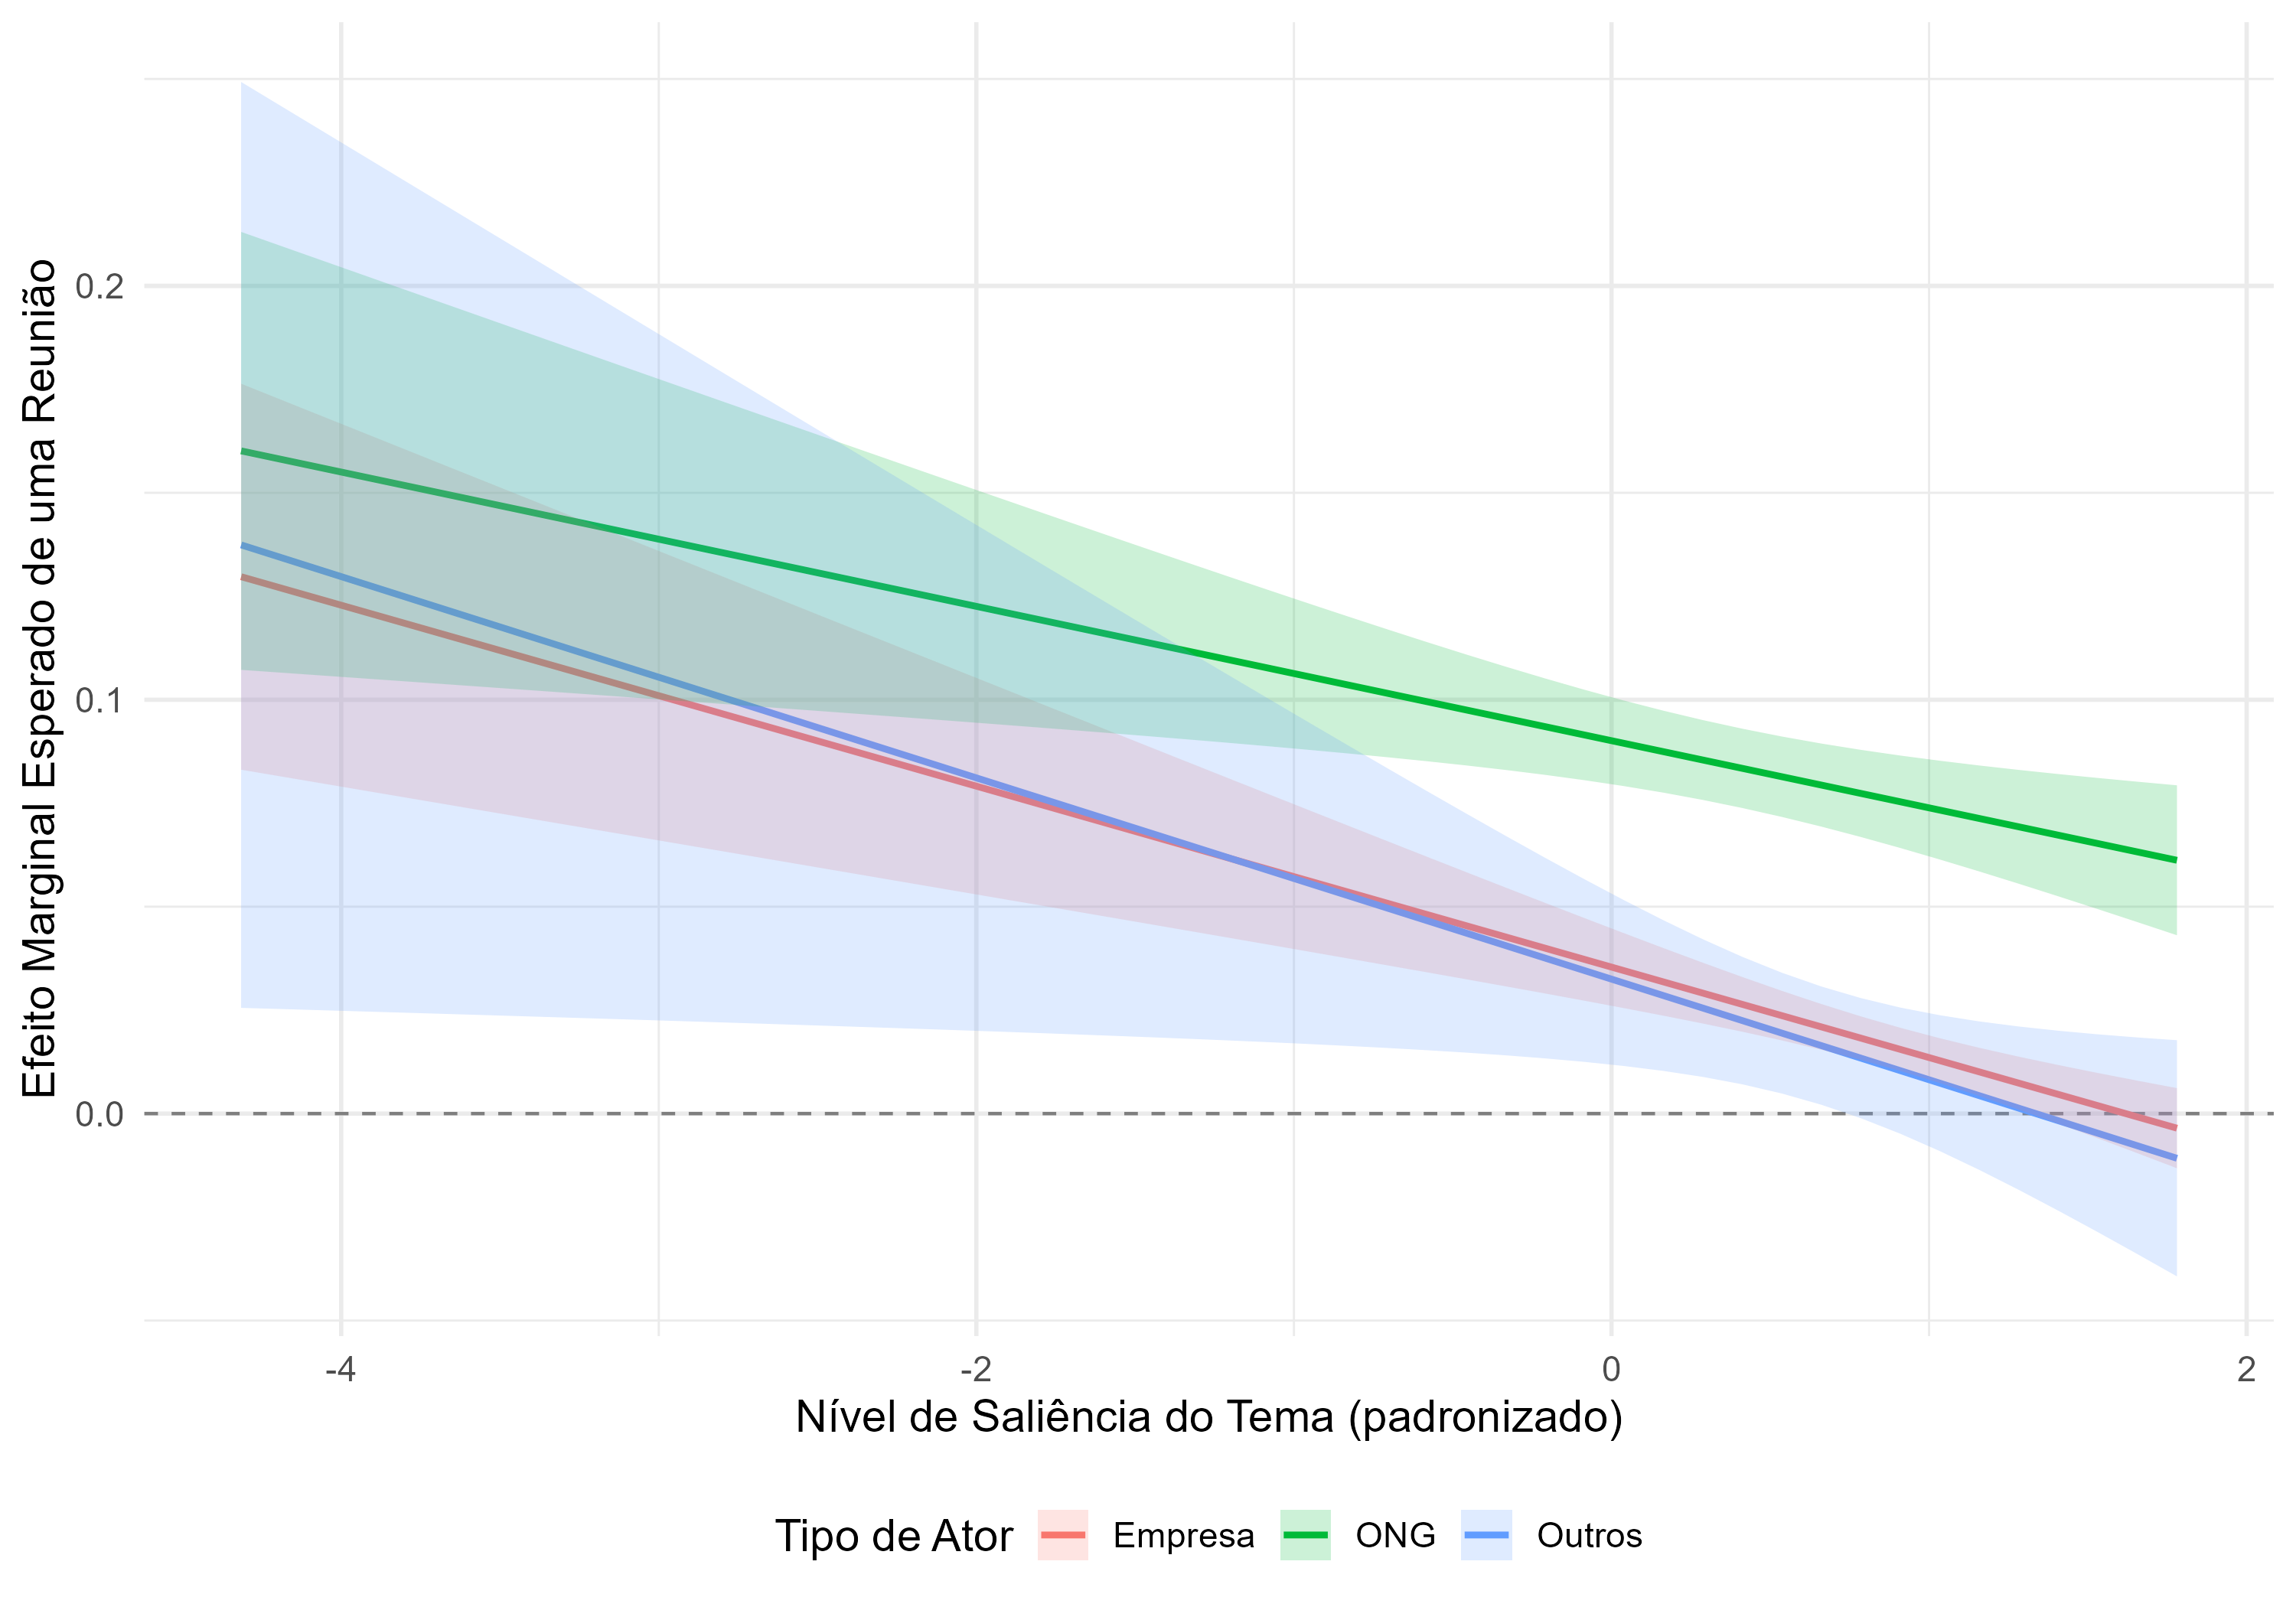
\includegraphics[width=\textwidth]{figures/h3_test/fig_h3_marginal_effects_manual.png}
    \caption{Efeito do Lobby Condicional à Saliência do Tema}
    \label{fig:h3_marginal_effects}
    \note{O gráfico exibe o efeito marginal esperado de uma única reunião sobre o número de perguntas parlamentares (eixo Y) em diferentes níveis de saliência do tema (eixo X). As linhas representam a estimativa para cada categoria de ator, e as áreas sombreadas correspondem aos intervalos de confiança de 95\%, calculados via bootstrap.}
\end{figure}

A análise revela um padrão complexo que contradiz parcialmente, mas também enriquece, a Hipótese 3. Contrariamente à expectativa de que o efeito das \acrshort{ong}s aumentaria com a saliência, observamos que o efeito marginal de uma reunião \textbf{diminui} para todos os grupos à medida que um tema se torna mais saliente (coeficiente negativo para todos os grupos nas variáveis de interação). Este achado está em forte alinhamento com a literatura, que sugere que a influência do lobby direto decresce quando a opinião pública e a atenção da mídia se intensificam, forçando os parlamentares a se alinharem a considerações eleitorais mais amplas \cite{mahoney_lobbying_2007, kollman1998outside}.

No entanto, a análise revela uma heterogeneidade crucial na taxa dessa diminuição. Três pontos principais se destacam na Figura \ref{fig:h3_marginal_effects}. Em temas de baixa saliência (à esquerda do gráfico), o efeito das \acrshort{ong}s é similar estatisticamente ao de empresas e outros atores. Isso pode ser observado pela intersecção das áreas sombreadas das linhas, que indicam o intervalo de confiança de 95\% das estimativas.
    
À medida que a saliência aumenta (movendo-se para a direita no gráfico), a vantagem comparativa das \acrshort{ong}s se acentua significativamente. O efeito do lobby de empresas e de outros atores decai rapidamente, enquanto o efeito das \acrshort{ong}s se mostra muito mais resiliente, diminuindo a uma taxa consideravelmente menor.
    
Em temas de alta saliência, onde a influência de empresas e outros grupos se torna estatisticamente indistinguível de zero (seus intervalos de confiança cruzam a linha pontilhada), o efeito das \acrshort{ong}s permanece positivo, robusto e estatisticamente significativo. É precisamente neste contexto de maior escrutínio público que a sua influência relativa se torna mais pronunciada.

Os resultados validam a Hipótese 3. Em temas de maior saliência, o lobby de organizações não empresariais é, de fato, mais eficaz em aumentar a atividade parlamentar em comparação com o lobby empresarial. A nuance importante é que essa maior eficácia não se manifesta como um aumento absoluto do efeito, mas sim como uma resiliência superior à pressão do escrutínio público, o que amplia a sua vantagem comparativa.

Esta descoberta dialoga diretamente com a teoria sobre os recursos do lobby e os incentivos parlamentares. Em temas de baixa saliência, os parlamentares, focados em seus objetivos de formulação de políticas (\textit{policy-seeking}), podem valorizar o subsídio informacional técnico fornecido por empresas. Contudo, quando um tema ganha visibilidade, os incentivos de reeleição (\textit{vote-seeking}) tornam-se dominantes \cite{mayhew2004congress}. Nesse contexto, alinhar-se a interesses empresariais pode ter um custo político elevado, enquanto responder a \acrshort{ong}s, que detêm maior capital de legitimidade \cite{bunea2018legitimacy}, reforça a imagem pública do parlamentar.

Os achados confirmam que a influência do lobby é altamente contextual e que, sob o escrutínio público, a vantagem se desloca para os atores percebidos como representantes de interesses mais amplos e difusos.
